\documentclass[../../main]{subfiles}

\begin{document}

\section{TikZデモ}
\label{sec:tikz}

多くの \code{usetikzlibrary} があらかじめ読み込まれているため\c 複雑な図もすぐに描画できます\p 以下は影付きノードや3Dグラフィックスなどのデモです\p 

\subsection{影付きノードと矢印}
\begin{figure}[H]
  \centering
  \begin{tikzpicture}[>=stealth, auto, node distance=3cm]
    \node [circle, draw, drop shadow, fill=blue!10] (A) {Node A};
    \node [rectangle, draw, drop shadow, fill=red!10, right of=A] (B) {Node B};
    
    \draw [->, thick] (A) edge[bend left] node {Next} (B);
    \draw [<-, thick, dashed] (A) edge[bend right] node[below] {Back} (B);
  \end{tikzpicture}
  \caption{TikZのライブラリ(shadows等)を用いたノードグラフ}
\end{figure}

\subsection{幾何学図形と交点・角度の計算}
\begin{figure}[H]
  \centering
  \begin{tikzpicture}[scale=1.5]
    % 座標の定義
    \coordinate (A) at (0,0);
    \coordinate (B) at (4,0);
    \coordinate (C) at (1.5, 3);
    
    % 三角形の描画
    \draw[thick, fill=blue!5] (A) -- (B) -- (C) -- cycle;
    
    % 各頂点のラベル
    \node[below left] at (A) {A};
    \node[below right] at (B) {B};
    \node[above] at (C) {C};
    
    % 角度の描画 (anglesライブラリ)
    \pic [draw, "$\alpha$", angle eccentricity=1.5] {angle = B--A--C};
    \pic [draw, "$\beta$", angle eccentricity=1.5] {angle = C--B--A};
    \pic [draw, "$\gamma$", angle eccentricity=1.5] {angle = A--C--B};

    % 垂線の計算 (calcライブラリ)
    \coordinate (D) at ($(A)!(C)!(B)$); % CからABへの垂線の足
    \draw[dashed, red, thick] (C) -- (D);
    \node[below] at (D) {D};
    
    % 直角記号
    \pic [draw, angle radius=3mm] {right angle = C--D--B};
  \end{tikzpicture}
  \caption{calcとanglesライブラリを用いた幾何学計算のデモ}
\end{figure}

\subsection{状態遷移図(オートマトン)}
\begin{figure}[H]
  \centering
  \begin{tikzpicture}[>=stealth, auto, node distance=2.5cm, on grid, thick]
    % 状態ノードの定義
    \node[state, initial, fill=gray!10] (q0) {$q_0$};
    \node[state, accepting, fill=gray!10] (q1) [right=of q0] {$q_1$};
    \node[state, fill=gray!10] (q2) [below=of q0] {$q_2$};
    \node[state, fill=gray!10] (q3) [below=of q1] {$q_3$};

    % 遷移の描画
    \path[->] 
      (q0) edge node {0} (q1)
           edge node[left] {1} (q2)
      (q1) edge[loop above] node {0} (q1)
           edge node {1} (q3)
      (q2) edge node {0} (q3)
           edge[loop below] node {1} (q2)
      (q3) edge[loop right] node {0, 1} (q3);
  \end{tikzpicture}
  \caption{automataライブラリを用いた状態遷移図のデモ}
\end{figure}

\subsection{数学関数のグラフ}
\begin{figure}[H]
  \centering
  \begin{tikzpicture}[>=stealth, xscale=1.5, yscale=1.5]
    % 軸の描画
    \draw[->] (-2.5, 0) -- (2.5, 0) node[right] {$x$};
    \draw[->] (0, -1.5) -- (0, 1.5) node[above] {$y$};
    
    % 目盛り
    \foreach \x in {-2,-1,1,2} \draw (\x, 0.05) -- (\x, -0.05) node[below] {$\x$};
    \foreach \y in {-1,1} \draw (0.05, \y) -- (-0.05, \y) node[left] {$\y$};
    \node[below left] at (0,0) {$O$};
    
    % グラフの描画
    \draw[color=red, thick, domain=-2.2:2.2, samples=100] plot (\x, {sin(\x r)}) node[right] {$\sin(x)$};
    \draw[color=blue, thick, dashed, domain=-2.3:2.3] plot (\x, {0.5*\x}) node[right] {$y = \frac{1}{2}x$};
  \end{tikzpicture}
  \caption{TikZ標準機能を用いた関数グラフの描画デモ}
\end{figure}

\subsection{マインドマップ}
\begin{figure}[H]
  \centering
  \begin{tikzpicture}[mindmap, grow cyclic, every node/.style=concept, concept color=teal!40,
    level 1/.append style={level distance=4cm, sibling angle=90},
    level 2/.append style={level distance=2.5cm, sibling angle=45}]
    
    \node {TikZ}
      child[concept color=orange!40] { node {2D}
        child { node {Geometry} }
        child { node {Graphs} }
      }
      child[concept color=blue!40] { node {3D}
        child { node {Perspective} }
      }
      child[concept color=green!40] { node {Diagrams}
        child { node {Automata} }
        child { node {Trees} }
      }
      child[concept color=purple!40] { node {Plots} };
  \end{tikzpicture}
  \caption{mindmapライブラリを用いたダイアグラムのデモ}
\end{figure}

\subsection{3D結晶構造描画}
\begin{figure}[H]
  \centering
  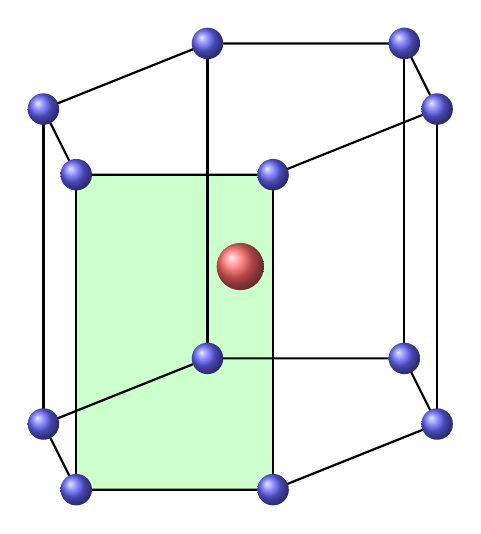
\begin{tikzpicture}
    % 下層の原子位置
    \coordinate[] (P11) at ( 2.5, 0, 0);
    \coordinate[] (P12) at ( 1.25, 0, 2.5 * 1.732 / 2);
    \coordinate[] (P13) at (-1.25, 0, 2.5 * 1.732 / 2);
    \coordinate[] (P14) at (-2.5, 0, 0);
    \coordinate[] (P15) at (-1.25, 0, -2.5 * 1.732 / 2);
    \coordinate[] (P16) at ( 1.25, 0, -2.5 * 1.732 / 2);

    % 上層の原子位置
    \coordinate[] (P21) at ( 2.5, 4, 0);
    \coordinate[] (P22) at ( 1.25, 4, 2.5 * 1.732 / 2);
    \coordinate[] (P23) at (-1.25, 4, 2.5 * 1.732 / 2);
    \coordinate[] (P24) at (-2.5, 4, 0);
    \coordinate[] (P25) at (-1.25, 4, -2.5 * 1.732 / 2);
    \coordinate[] (P26) at ( 1.25, 4, -2.5 * 1.732 / 2);

    % 特定の面の描画 (緑色で強調)
    \draw[fill=green!20, draw=none] (P12) -- (P13) -- (P23) -- (P22) -- cycle;

    % 枠線の描画
    \draw[thick] (P11) -- (P12) -- (P13) -- (P14) -- (P15) -- (P16) -- cycle; % 下面
    \draw[thick] (P21) -- (P22) -- (P23) -- (P24) -- (P25) -- (P26) -- cycle; % 上面
    
    % 縦の結合線
    \draw[thick] (P11) -- (P21);
    \draw[thick] (P12) -- (P22);
    \draw[thick] (P13) -- (P23);
    \draw[thick] (P14) -- (P24);
    \draw[thick] (P15) -- (P25);
    \draw[thick] (P16) -- (P26);

    % 中心の原子(例)
    \shade[ball color=red!60] (0, 2, 0) circle (0.3);

    % 各頂点に原子を配置
    \foreach \pt in {P11,P12,P13,P14,P15,P16,P21,P22,P23,P24,P25,P26} {
      \shade[ball color=blue!60] (\pt) circle (0.2);
    }
  \end{tikzpicture}
  \caption{TikZによる3D結晶構造(六方最密構造)の描画デモ}
\end{figure}

\subsection{論理回路}
\begin{figure}[H]
  \centering
  \begin{tikzpicture}[circuit logic US, every circuit symbol/.style={thick}]
    % 入力
    \node (x) at (0, 1) {$x$};
    \node (y) at (0, 0) {$y$};
    
    % ゲート
    \node[and gate, inputs={nn}] (and1) at (2, 0.5) {};
    \node[not gate] (not1) at (2, -0.5) {};
    
    % 入力からゲートへの配線
    \draw (x.east) -- ++(0.5,0) |- (and1.input 1);
    \draw (y.east) -- ++(0.3,0) |- (and1.input 2);
    \draw (y.east) -- ++(0.3,0) |- (not1.input);
    
    % 出力
    \draw (and1.output) -- ++(0.5,0) node[right] {$x \land y$};
    \draw (not1.output) -- ++(0.5,0) node[right] {$\lnot y$};
  \end{tikzpicture}
  \caption{circuits.logic.USライブラリを用いた論理回路デモ}
\end{figure}

\subsection{木構造(ツリー)}
\begin{figure}[H]
  \centering
  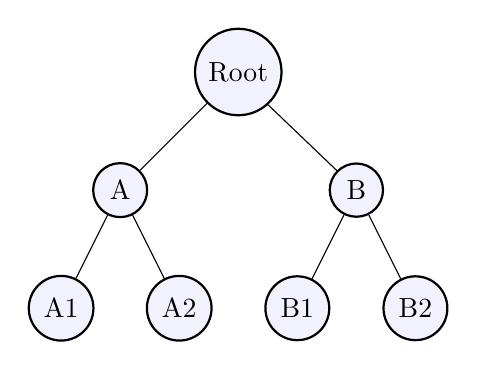
\begin{tikzpicture}[
    level 1/.style={sibling distance=3cm},
    level 2/.style={sibling distance=1.5cm},
    every node/.style={circle, draw, align=center, thick, fill=blue!5}
  ]
    \node {Root}
      child { node {A}
        child { node {A1} }
        child { node {A2} }
      }
      child { node {B}
        child { node {B1} }
        child { node {B2} }
      };
  \end{tikzpicture}
  \caption{treesライブラリを用いた木構造のデモ}
\end{figure}

\subsection{部分拡大図}
\begin{figure}[H]
  \centering
  % spy using outlinesに設定を追加
  \begin{tikzpicture}[spy using outlines={circle, magnification=3, size=2.5cm, connect spies}]
    % 元の図形
    \begin{scope}
      \draw[step=0.2cm, gray!30, thin] (0,0) grid (3,2);
      \draw[thick, color=blue] (0,0) sin (1.5, 1) cos (3, 0);
      \node[below] at (1.5, -0.2) {Original Plot};
    \end{scope}
    
    % spy（拡大先と拡大範囲の指定）
    % 座標(1.5, 1)付近を拡大し、それを座標(5, 1)に配置
    \spy[red] on (1.5, 1) in node at (5, 1);
  \end{tikzpicture}
  \caption{spyライブラリを用いた部分拡大のデモ}
\end{figure}

\subsection{パターンの塗りつぶし}
\begin{figure}[H]
  \centering
  \begin{tikzpicture}
    % 斜線（右上上がり）
    \draw[pattern=north east lines, pattern color=blue] (0,0) rectangle (2,2);
    \node[below] at (1, -0.2) {north east lines};

    % クロスハッチ
    \draw[pattern=crosshatch, pattern color=red] (3,0) rectangle (5,2);
    \node[below] at (4, -0.2) {crosshatch};

    % ドット
    \draw[pattern=crosshatch dots, pattern color=green!60!black] (6,0) rectangle (8,2);
    \node[below] at (7, -0.2) {crosshatch dots};
  \end{tikzpicture}
  \caption{patternsライブラリを用いたメッシュ等の塗りつぶしデモ}
\end{figure}

\end{document}
